\documentclass{article}\usepackage[]{graphicx}\usepackage[]{color}
%% maxwidth is the original width if it is less than linewidth
%% otherwise use linewidth (to make sure the graphics do not exceed the margin)
\makeatletter
\def\maxwidth{ %
  \ifdim\Gin@nat@width>\linewidth
    \linewidth
  \else
    \Gin@nat@width
  \fi
}
\makeatother

\definecolor{fgcolor}{rgb}{0.345, 0.345, 0.345}
\newcommand{\hlnum}[1]{\textcolor[rgb]{0.686,0.059,0.569}{#1}}%
\newcommand{\hlstr}[1]{\textcolor[rgb]{0.192,0.494,0.8}{#1}}%
\newcommand{\hlcom}[1]{\textcolor[rgb]{0.678,0.584,0.686}{\textit{#1}}}%
\newcommand{\hlopt}[1]{\textcolor[rgb]{0,0,0}{#1}}%
\newcommand{\hlstd}[1]{\textcolor[rgb]{0.345,0.345,0.345}{#1}}%
\newcommand{\hlkwa}[1]{\textcolor[rgb]{0.161,0.373,0.58}{\textbf{#1}}}%
\newcommand{\hlkwb}[1]{\textcolor[rgb]{0.69,0.353,0.396}{#1}}%
\newcommand{\hlkwc}[1]{\textcolor[rgb]{0.333,0.667,0.333}{#1}}%
\newcommand{\hlkwd}[1]{\textcolor[rgb]{0.737,0.353,0.396}{\textbf{#1}}}%

\usepackage{framed}
\makeatletter
\newenvironment{kframe}{%
 \def\at@end@of@kframe{}%
 \ifinner\ifhmode%
  \def\at@end@of@kframe{\end{minipage}}%
  \begin{minipage}{\columnwidth}%
 \fi\fi%
 \def\FrameCommand##1{\hskip\@totalleftmargin \hskip-\fboxsep
 \colorbox{shadecolor}{##1}\hskip-\fboxsep
     % There is no \\@totalrightmargin, so:
     \hskip-\linewidth \hskip-\@totalleftmargin \hskip\columnwidth}%
 \MakeFramed {\advance\hsize-\width
   \@totalleftmargin\z@ \linewidth\hsize
   \@setminipage}}%
 {\par\unskip\endMakeFramed%
 \at@end@of@kframe}
\makeatother

\definecolor{shadecolor}{rgb}{.97, .97, .97}
\definecolor{messagecolor}{rgb}{0, 0, 0}
\definecolor{warningcolor}{rgb}{1, 0, 1}
\definecolor{errorcolor}{rgb}{1, 0, 0}
\newenvironment{knitrout}{}{} % an empty environment to be redefined in TeX

\usepackage{alltt}

\usepackage{fancyhdr} % Required for custom headers
\usepackage{lastpage} % Required to determine the last page for the footer
\usepackage{extramarks} % Required for headers and footers
\usepackage{graphicx} % Required to insert images
\usepackage{hyperref}
\usepackage{amsmath} %for binomial pdf
\usepackage{parskip} % so that there's space bw paragraphs
\usepackage{float}

% Margins
\topmargin=-0.45in
\evensidemargin=0in
\oddsidemargin=0in
\textwidth=6.5in
\textheight=9.0in
\headsep=0.25in 

\linespread{1.1} % Line spacing

% Set up the header and footer
\pagestyle{fancy}
\lhead{STAT 532: Bayes} % Top left header
\chead{HW 1} % Top center header
\rhead{Andrea Mack} % Top right header
\lfoot{09/17/2016} % Bottom left footer
\cfoot{} % Bottom center footer
\rfoot{Page\ \thepage\ of\ \pageref{LastPage}} % Bottom right footer
\renewcommand\headrulewidth{0.4pt} % Size of the header rule
\renewcommand\footrulewidth{0.4pt} % Size of the footer rule

\setlength\parindent{0pt} % Removes all indentation from paragraphs
\setlength\parskip{0.5cm}
\restylefloat{table}

%----------------------------------------------------------------------------------------
%	DOCUMENT STRUCTURE COMMANDS
%	Skip this unless you know what you're doing
%----------------------------------------------------------------------------------------

% Header and footer for when a page split occurs within a problem environment
\newcommand{\enterProblemHeader}[1]{
\nobreak\extramarks{#1}{#1 continued on next page\ldots}\nobreak
\nobreak\extramarks{#1 (continued)}{#1 continued on next page\ldots}\nobreak
}

% Header and footer for when a page split occurs between problem environments
\newcommand{\exitProblemHeader}[1]{
\nobreak\extramarks{#1 (continued)}{#1 continued on next page\ldots}\nobreak
\nobreak\extramarks{#1}{}\nobreak
}


%----------------------------------------------------------------------------------------%
\IfFileExists{upquote.sty}{\usepackage{upquote}}{}
\begin{document}


%----------------------------------------------------------------------------------------
%	Talk Description
%----------------------------------------------------------------------------------------
\begin{enumerate}
\item %one
{\it (24 pts) Describe the differences between Bayesian and classical inference. Include a discussion on confidence and credible intervals.}

\section*{\small{Interval Estimates}}

Dr. Hoff describes Bayesian inference as, ``the process of inductive learning via Bayes' rule" (which is different from the view Gelman and Shalizi (2013) take on Bayesian inference). Using Bayes' rule, we can make probablistic statements about parameters, after incorporating information from the sample. Dr. Hoff says that probabilities are synonomous with information. Bayesian inference subsets the prior information about the parameters into the space of the observed data, and concludes with updated information about the parameters in that subseted parameter space.

In Bayesian inference, we have to find a reasonable prior distribution, complete with it's parameters and know the distribution of the data conditioned on the parameters. In comparison to classical inference, where we do not need to know or guess  prior distribution. A benefit of Bayesian inference is that we can make credible intervals for the parameters. The credibility of a credible interval is the probability that the parameter is in the interval.

To make inference about the values for the parameter that are plausible in classical inference, we make confidence intervals. The confidence of a confidence interval is the long run percentage of confidence intervals that are expected to contain the parameter. This means that if I take many, many samples and create corresponding confidence intervals for each sample, that in the long run, the confidence level is the percentage of confidence intervals that are expected to contain the true parameter.

\section*{\small{Testing and Modeling}}

Gelman and Shelizi (2013) discuss classical statistics as ``falsification". In classical inference, we make null and alternative hypotheses about parameters or models, and based on the probability of the observed result or more extreme under the null determine the strength of evidence against the null. In classical inference, we can not say that the null hypothesis is true, only the strength of evidence against the null. For example, we could have two hypothesis tests, (1) $H_{o}: \theta = 0$ and $H_{a}: \theta \neq 0$ and (2) $H_{o}: \theta = 0.5$ and $H_{a}: \theta \neq 0.5$. If both tests results in a high pvalue and suppose that in classical inference we could accept the null, we would conclude both that $\theta$ = 0 and $\theta$ = 0.5, but $\theta$ can only take on one value. In classical hypothesis testing, we can only say there was no evidence that another model or parameter was better than that assumed. This is versus probabilistic statements {\it for} models we can make using Bayesian inference. Gelman and Shalizi (2013) also discuss the importance of model checking in Bayesian inference, as seeing {\it where} the model may be less accurate versus having the end point goal of finding a posterior distribution. To me it seems that model checking would be important in both classical and bayesian inference.
\newpage

\item %two
{\it (1 pt) Do you consider yourself a Bayesian or classical Statistician?}

For now, I like the idea of Bayesian inference because it is intuitive and realistic in how many people think. For example, it's hard to think about what sort of assurance we should put in a long run accuracy (confidence level) in a single case. Both classical and bayesian inference seem to have some subjectivity (sample size and priors). 

%This extension may be a stretch, but in my career as a statistician, I would rather control the probability I come to correct conclusions in each individual study I work on rather than If in my career I do classical inference 1000 times using 95\% confidence  doubt that even in my lifetime I will near the asymptote needed for classical inference to reach a desired confidence level to know ``how well" I will have done in the long run of my career.


\item %three
{\it Assume you are hired by Bridger Bowl to compute the probability that an MSU student either skis (or snowboards). }
\begin{enumerate} 
\item %a
{\it (10 pts) If binary data are collected from 300 students, what is the sampling model for this research question? Please name the distribution and write out the corresponding sampling distribution.}

WHERE $X_{i}$ = 1 IF SKI/SNOWBOARD 0 ELSE

Let x = the number of students that either ski or snowboard, then x $\sim$ BIN(300, $\theta$).


f(x\vert$\theta$) = $\binom{300}{x}$ $\theta^{x}(1-\theta)^{300-x}$ \cdot $I(x)_{[0,1,...,300]}$


\item %b
{\it (10 pts) Use a prior distribution from the Beta distribution and create a plot/histogram from this distribution. Why did you choose the $\alpha$ and $\beta$ values for this prior distribution? Hint: R code}

The hinted R code used values of 0.1 for both $\alpha$ and $\beta$. Using those values, that means we would expect half of the students to ski or snowboard and that the distribution of the proportion that ski or snowboard would be similar to the plot below.

First, I would guess that more than half of MSU students have skiied or snowboarded before. I would guess this is around 65\%. However, there are many distributions that would yield an expected 65\% of skiiers or snowboarders. Below are plotted several with $\alpha$ and $\beta$ combinations, all with an expected value of 0.65, with $\alpha$ and $\beta$ ranging from 0.1 to 100 and from 0.0534 to 53.85, respectively. I came up with the $\alpha$ and $\beta$ values by making an equally spaced sequence from 0.1 to 100 of length 20 $\alpha$, solving for $\beta$ that would make the expected proportion equal to 0.65, and then plotting each of these beta distributions.

The distribution that I think visually is most reasonable is shown in red, with $\alpha$ = 47.42 and $\beta$ = 25.53, although there is not much of a difference in the distributions with parameters near to these values. The distribution I chose suggests that on average, 65\% of MSU students ski/snowboard, and it is most likely that between about 50\% and 80\% of MSU students ski/snowboard.



\begin{figure}[htbp]
\begin{knitrout}
\definecolor{shadecolor}{rgb}{0.969, 0.969, 0.969}\color{fgcolor}
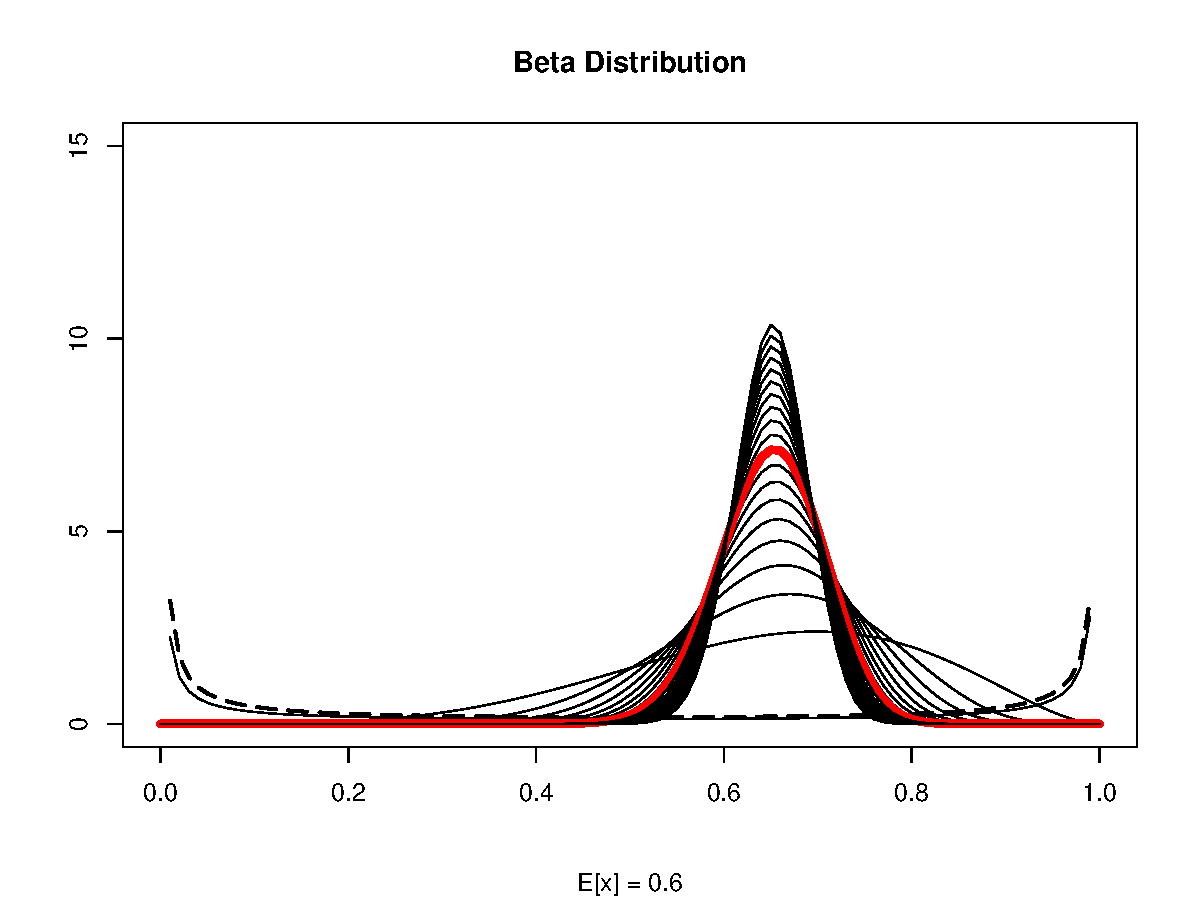
\includegraphics[width=\maxwidth]{figure/3bx-1} 

\end{knitrout}


\end{figure}

The BETA(0.1,0.1) is plotted with the dashed line. The expected value of any beta distribution with $\alpha = \beta$ is symmetric about $\frac{1}{2}$. You might choose the parameters on the prior beta distribution to be equal if you believe that the probability distribution of $\theta$ taking on each of the possible values is symmetric about $\frac{1}{2}$. By setting the prior parameters both equal to 0.1, you are assuming it is most likely that either there is no chance of students skiing or snowboarding, or there is a high chance of students skiing or snowboarding.

\newpage
{\bf Why to choose $\alpha$ and $\beta$:}
It is very rare that we know the parameter (here $\theta$, the true probability of a student snowboarding or skiing). We know that for probabilities, the beta distribution, which has domain (0,1) is often reasonable. However, to use the beta distribution to model the probability of $\theta$ taking on certain values, we have to make more assumptions about the probability distribution of $\theta$, we have to set the parameters of the beta distribution. In class we discussed that $\alpha$ can be interpretted as the expected number of students that ski or snowboard, and $\beta$ is the expected total number of students, which is a place to start. However, many beta distributions have expectations of $\frac{1}{2}$, and just because we may expect the probability of a person skiing or snowboarding to be $\frac{1}{2}$, that does not tell us about the probability of $\theta$ falling in any interval. It is not clear to me about how to set these parameters or how to account for the added uncertainty with making assumptions about the prior parameters. Note that as we discussed in class, the BETA(1,1) is the UNIF(0,1) distribution which would mean essentially that the prior is uninformative about which intervals are likely for $\theta$.

\item %c
{\it (15 pts) Assume 234 of the sample MSU students claim to either ski or snowboard. Compute the posterior distribution, $p(\theta|Y)$ where $\theta$ is the probability of MSU student skiing and Y is the observed responses. }

$\theta$ $\sim$ BETA($\alpha,\beta$) and  $Y|\theta \sim$ BIN(300,$\theta$)

$p(\theta|Y)$ = $\frac{p(Y|\theta)*p(\theta)}{p(Y)}$:

$p(Y)$ = $\int_{\mathcal{\theta}} \binom{300}{Y} \cdot \theta^{Y} \cdot (1-\theta)^{300-Y} \cdot \frac{\Gamma(\alpha)\Gamma(\beta)}{\Gamma(\alpha+\beta)} \cdot \theta^{\alpha-1}(1-\theta)^{\beta-1} d{\theta}$

= $c^{*} \cdot \int_{\mathcal{\theta}} \theta^{Y+\alpha-1}(1-\theta)^{300-Y+\beta-1} d{\theta}$

where $c^{*}$ = $\binom{300}{Y} \cdot \frac{\Gamma(\alpha)\Gamma(\beta)}{\Gamma(\alpha+\beta)}$

then if $c^{**}$ = $c^{*} \cdot \frac{\Gamma(\alpha+\beta+300)}{\Gamma(Y+\alpha)\Gamma(300-Y+\beta)}$

$p(Y)$ = $c^{**} \cdot 1$

now, $p(\theta|Y)$ = $\frac{p(Y|\theta)*p(\theta)}{p(Y)}$ = $\frac{\binom{300}{Y} \cdot \theta^{Y} \cdot (1-\theta)^{300-Y} \cdot \frac{\Gamma(\alpha)\Gamma(\beta)}{\Gamma(\alpha+\beta)} \cdot \theta^{\alpha-1}(1-\theta)^{\beta-1}}{\binom{300}{Y} \cdot \frac{\Gamma(\alpha)\Gamma(\beta)}{\Gamma(\alpha+\beta)} \cdot \frac{\Gamma(\alpha+\beta+300)}{\Gamma(Y+\alpha)\Gamma(300-Y+\beta)}}$

= $\frac{\theta^{Y+\alpha-1} \cdot (1-\theta)^{300-Y+\beta-1}}{\frac{\Gamma(\alpha+\beta+300)}{\Gamma(Y+\alpha)\Gamma(300-Y+\beta)}}$

= $\frac{\Gamma(Y+\alpha)\Gamma(234-Y+\beta)}{\Gamma(\alpha+\beta+300)} \cdot \theta^{Y+\alpha-1} \cdot (1-\theta)^{300-Y+\beta-1}$

which is the pdf of a BETA($Y+\alpha$, $300-Y+\beta$) distribution.

If the prior of $\theta$ is BETA($\alpha$, $\beta$), the posterior is BETA($\alpha+x, \alpha+\beta+N-y$) where N is the total sample size.

$\therefore$ $\theta|x \sim BETA(47.42+234,47.42+25.53+300-234)$ $\implies$ $\theta|x \sim BETA(281.42,138.95)$

and again recall that $\theta \sim BETA(47.42,25.53)$. 

\item %d
{\it (10 pts) Plot the posterior distribution computed in part (c).}
The posterior is plotted in black below, and the prior in red. The data change the beliefs about the posterior distribution substantially.

\begin{center}
\begin{knitrout}
\definecolor{shadecolor}{rgb}{0.969, 0.969, 0.969}\color{fgcolor}
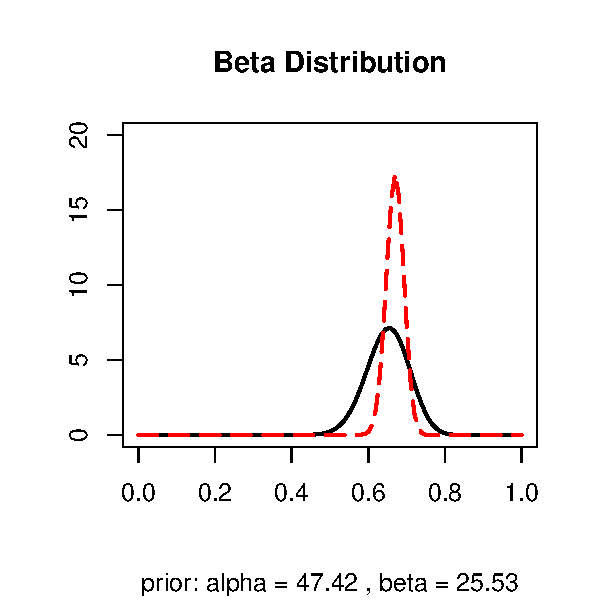
\includegraphics[width=\maxwidth]{figure/3d-1} 

\end{knitrout}
\end{center}

\item %e
{\it (10 pts) Compute a 95\% credible interval for $\theta$. }

There is a 95\% chance that theta is between 0.5378032 and 0.7544716 .

\end{enumerate}
\newpage


\item %4
{\it Hoff Exercise 2.1 - Marginal and conditional probability: The social mobility data from Section 2.5 gives a joint probability distribution on $(Y_{1}, Y_{2})$ = (father's occupation, son's occupation). Using this joint distribution, calculate the following distribution:



\begin{enumerate}
\item %a 
{\it (5 pts) the marginal probability distribution of a father\textsc{\char13}s occupation}

% latex table generated in R 3.3.1 by xtable 1.8-2 package
% Fri Sep 16 12:25:17 2016
\begin{table}[ht]
\centering
\begin{tabular}{rrrrrrr}
  \hline
 & farm & operatives & craftsmen & sales & professional & father.total \\ 
  \hline
farm & 0.018 & 0.035 & 0.031 & 0.008 & 0.018 & 0.110 \\ 
  operatives & 0.002 & 0.112 & 0.064 & 0.032 & 0.069 & 0.279 \\ 
  craftsmen & 0.001 & 0.066 & 0.094 & 0.032 & 0.084 & 0.277 \\ 
  sales & 0.001 & 0.018 & 0.019 & 0.010 & 0.051 & 0.099 \\ 
  professional & 0.001 & 0.029 & 0.032 & 0.043 & 0.130 & 0.235 \\ 
  son.total & 0.023 & 0.260 & 0.240 & 0.125 & 0.352 & 1.000 \\ 
   \hline
\end{tabular}
\end{table}
% latex table generated in R 3.3.1 by xtable 1.8-2 package
% Fri Sep 16 12:25:17 2016
\begin{table}[ht]
\centering
\begin{tabular}{rrrrrrr}
  \hline
 & farm & operatives & craftsmen & sales & professional & else \\ 
  \hline
father's marginal pdf & 0.11 & 0.28 & 0.28 & 0.10 & 0.24 & 0.00 \\ 
   \hline
\end{tabular}
\end{table}



\item %b
{\it (5 pts) the marginal probability distribution of a sons occupation}

% latex table generated in R 3.3.1 by xtable 1.8-2 package
% Fri Sep 16 12:25:17 2016
\begin{table}[ht]
\centering
\begin{tabular}{rrrrrrr}
  \hline
 & farm & operatives & craftsmen & sales & professional & else \\ 
  \hline
son's marginal pdf & 0.02 & 0.26 & 0.24 & 0.12 & 0.35 & 0.00 \\ 
   \hline
\end{tabular}
\end{table}

\item % c 
{\it (5 pts) the conditional distribution of a son's occupation, given that the father is a farmer}

\begin{table}[H]
\centering
\begin{tabular}{rrrrrrr}
  \hline
 & farm & operatives & craftsmen & sales & professional & else \\ 
  \hline
son's pdf $|$ father = farmer & 0.164 & 0.318 & 0.282 & 0.073 & 0.164 & 0 \\ 
   \hline
\end{tabular}
\end{table}




\item %d 
{\it (5 pts) the conditional distribution of a father's occupation, given that the son is a farmer}

\begin{table}[H]
\centering
\begin{tabular}{rrrrrrr}
  \hline
 & farm & operatives & craftsmen & sales & professional & else \\ 
  \hline
father's pdf $|$ son = farmer & 0.783 & 0.087 & 0.043 & 0.043 & 0.043 & 0 \\ 
   \hline
\end{tabular}
\end{table}



\end{enumerate}


\end{enumerate}




\end{document}
